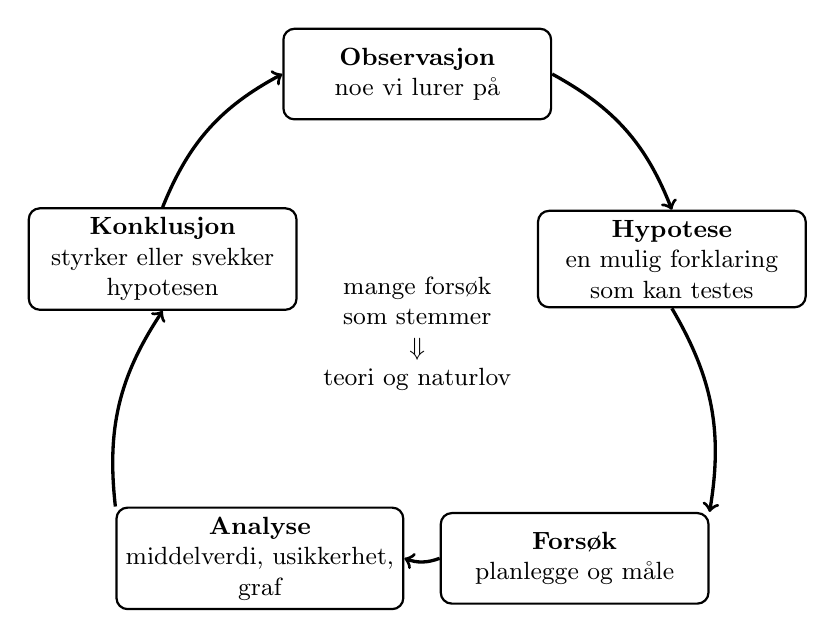
\begin{tikzpicture}[
  boks/.style={draw,thick,rounded corners=4pt,align=center,minimum width=3.4cm,minimum height=1.15cm,font=\small},
  pil/.style={->,very thick}]
\def\R{3.4}
\node[boks] (o) at (90:\R)  {\textbf{Observasjon}\\noe vi lurer på};
\node[boks] (h) at (18:\R)  {\textbf{Hypotese}\\en mulig forklaring\\som kan testes};
\node[boks] (f) at (-54:\R) {\textbf{Forsøk}\\planlegge og måle};
\node[boks] (a) at (-126:\R){\textbf{Analyse}\\middelverdi, usikkerhet,\\graf};
\node[boks] (m) at (162:\R) {\textbf{Konklusjon}\\styrker eller svekker\\hypotesen};
\draw[pil] (o.east) to[bend left=20] (h.north);
\draw[pil] (h.south) to[bend left=20] (f.north east);
\draw[pil] (f.west) to[bend left=20] (a.east);
\draw[pil] (a.north west) to[bend left=20] (m.south);
\draw[pil] (m.north) to[bend left=20] (o.west);
\node[align=center,font=\small] at (0,0.1) {mange forsøk\\som stemmer\\$\Downarrow$\\teori og naturlov};
\end{tikzpicture}
